\documentclass[letterpaper,12pt,leqno]{article}
\usepackage{paper1}
\usepackage[utf8]{inputenc}
\usepackage{hyperref}
\usepackage{url}
\usepackage{natbib}
\usepackage{float}
% 全局设置所有 itemize 环境的首行缩进

\usepackage{longtable}

% Enter paper title:
\hypersetup{pdftitle={Paper Title}}
% Enter permanent URL to paper
\available{https://github.com/pmichaillat/latex-paper}
% Enter BibTeX file with references:
% Enter PDF file with figures here:
\newcommand{\pdf}{figures.pdf}

\begin{document}
	
	\section{Task 1}\label{task-1}
	
	\subsection{a)}
	
	\begin{enumerate}
		\def\labelenumi{\arabic{enumi}.}
		\item
		Location of the new station
	\end{enumerate}
	
	The new Shepshed station is situated in the eastern suburbs of the town, an area with few residential buildings. This location avoids the high demolition costs usually seen with urban station construction. Importantly, its position allows easy access to most of the town within a 2000-meter radius(Figure \ref{fig:radius}), making it an ideal spot for the station. 
	
	\begin{figure}[H]
		\centering
		\includegraphics[width=0.6\linewidth]{digimap_roam.jpg}
		\caption{Location of the new station}
		\label{fig:radius}
	\end{figure}
		
	\begin{enumerate}
		\setcounter{enumi}{1}
		\item
		Route direction
	\end{enumerate}
	
	The proposed route shown in red in Figure \ref{fig:outline} bypasses Loughborough to the north. This detour not only extends the journey but also involves navigating challenging elevations in the northwest, which significantly raises construction costs due to the required excavation and filling works.
 
	However, this route minimizes disruptions to the urban road network, aligning with key stakeholder expectations. Importantly, it enhances operational efficiency by eliminating the need for speed reductions at Loughborough Central Station, which is crucial for maintaining optimal transit times. This alignment represents a deliberate trade-off, prioritizing operational and community benefits over the increased direct costs and construction complexities.
	
	\begin{figure}[H]
		\centering
		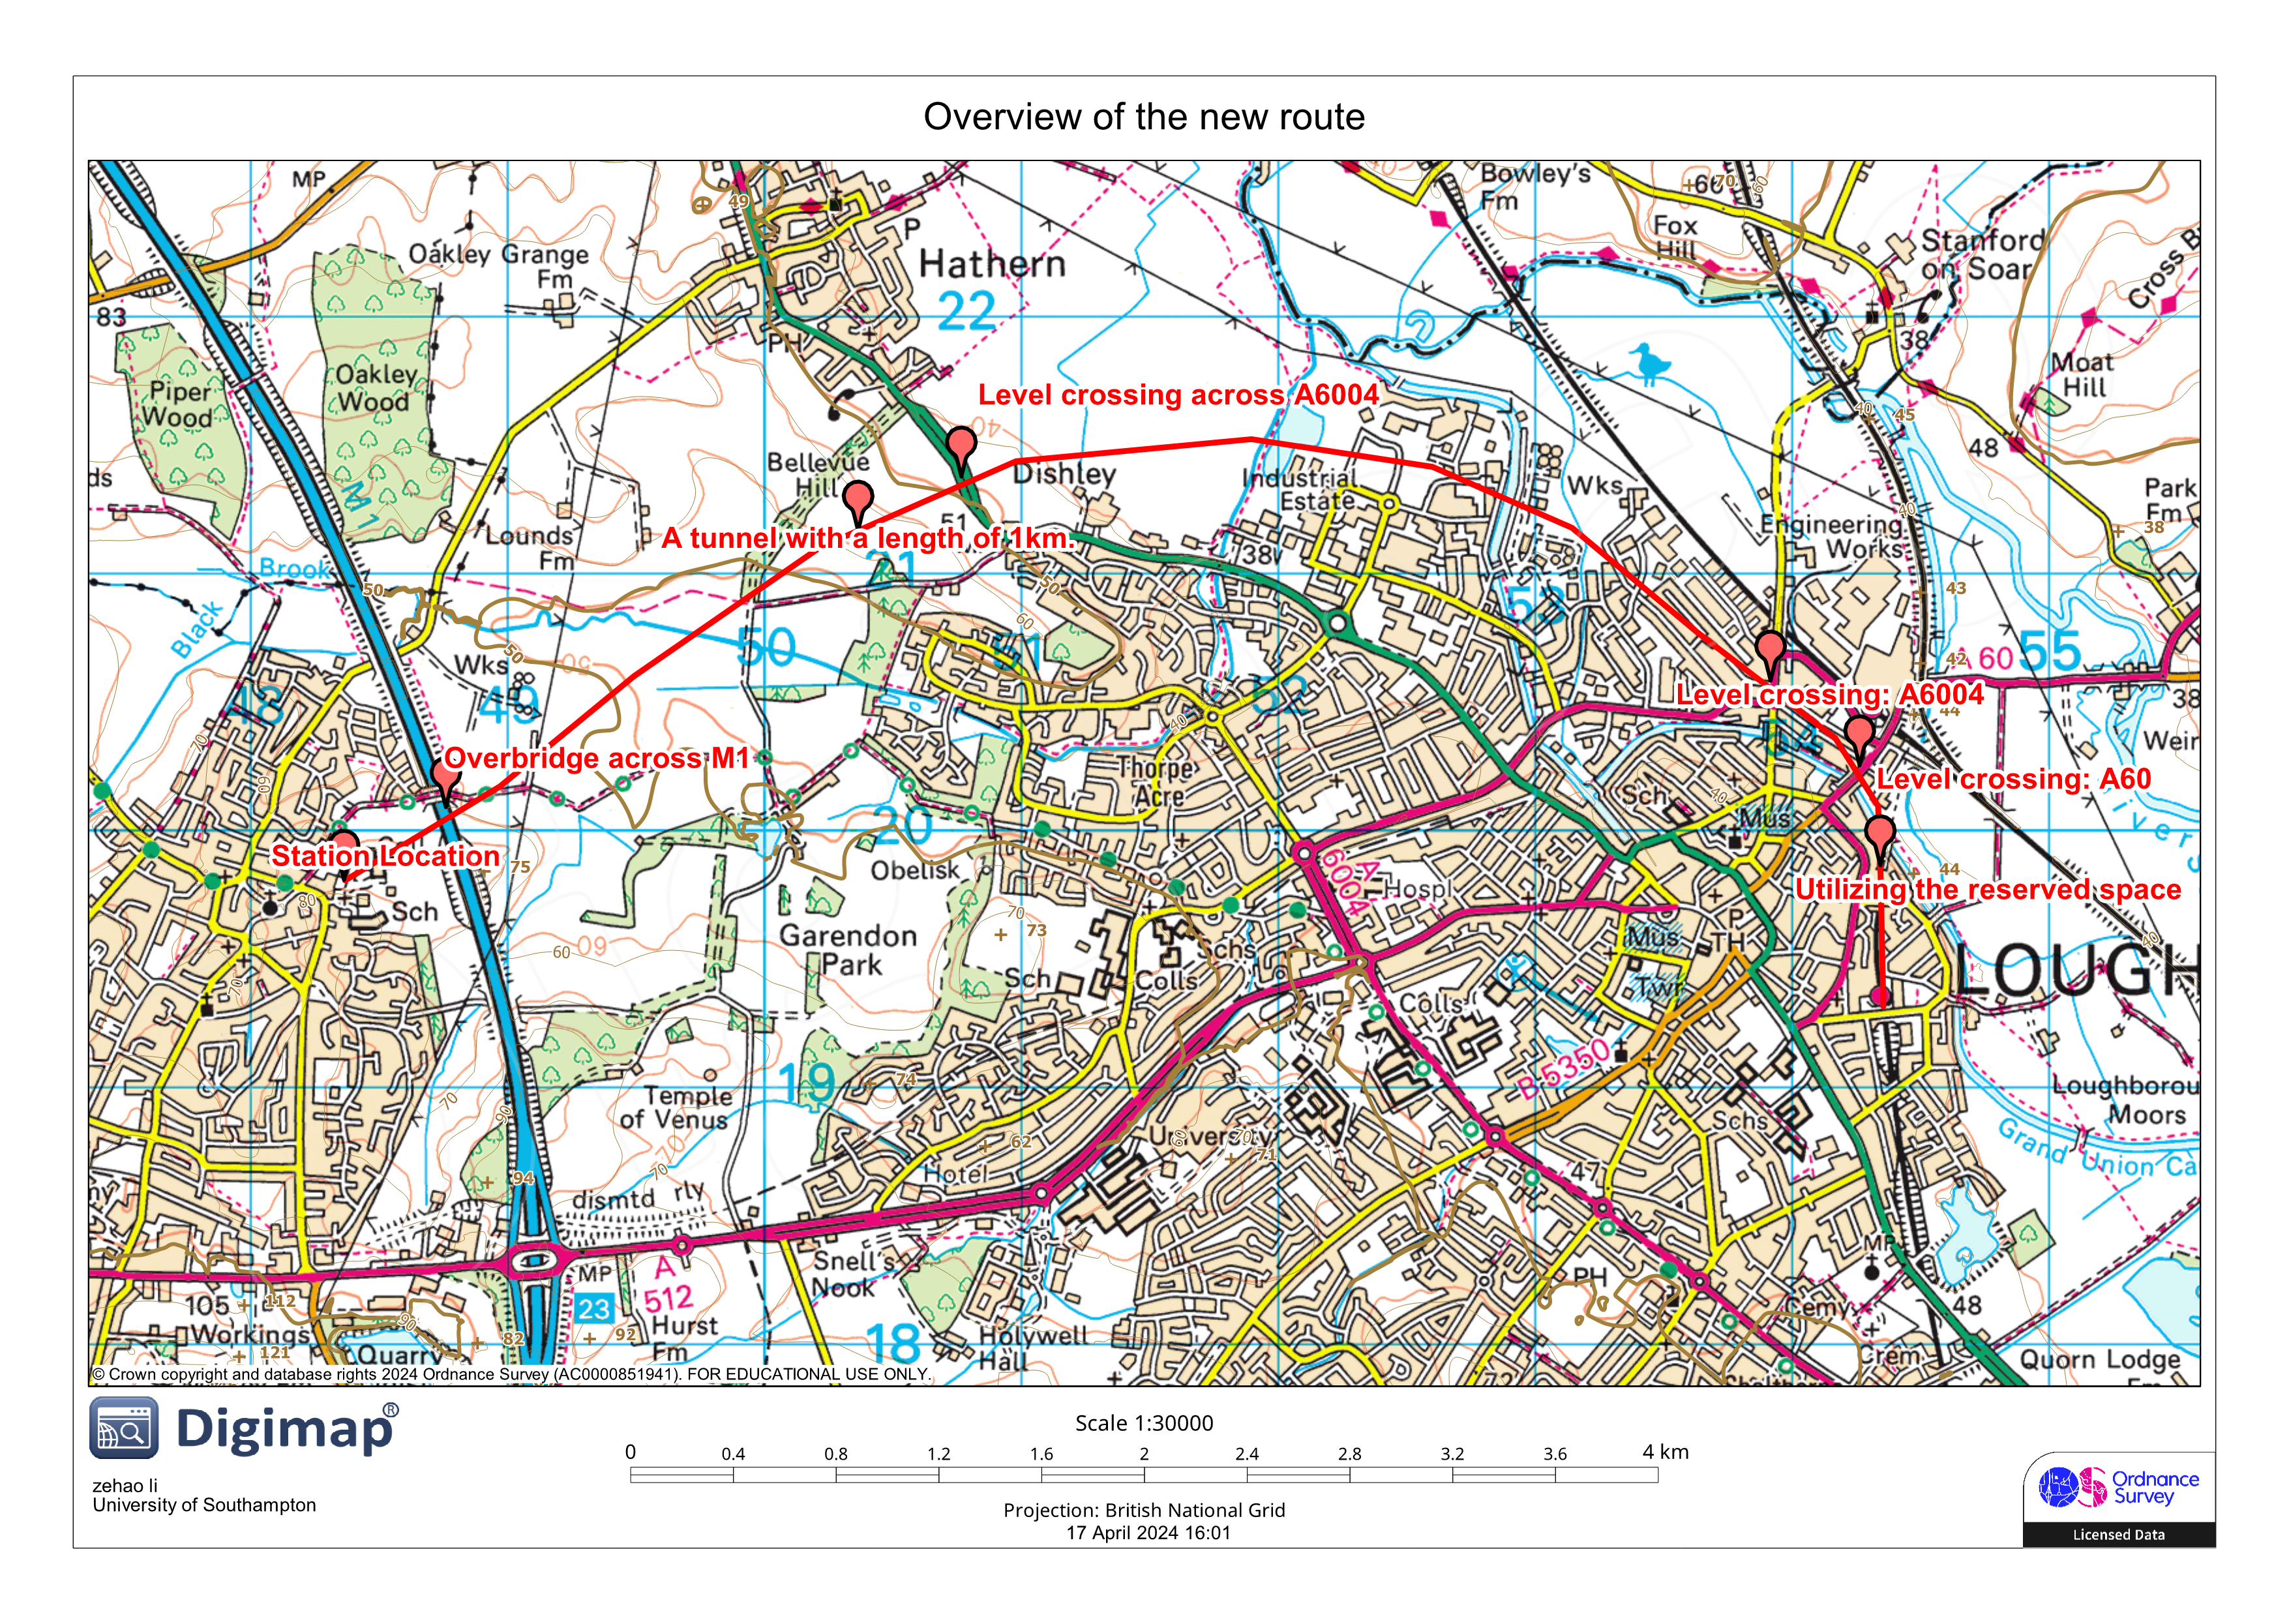
\includegraphics[width=\linewidth]{overview.png}
		\caption{the outline of the new route}
		\label{fig:outline}
	\end{figure}
	
	\begin{enumerate}
		\setcounter{enumi}{2}
		\item
		Key control points
	\end{enumerate}
	
	The design incorporates two types of control points to seamlessly
	integrate with existing infrastructure:
	
	
	\textbf{At Road Intersections}: Considering the number of people served by this route and the potential benefits, the high cost of excessively using bridges might lead to wastage. Therefore, for this project, when crossing roads like A60 and A6004, it uses level crossings(Figure \ref{fig:level crossing}). The service interval of this route indicates that these roads are blocked an average of three times per hour, which has a minimal impact on traffic flow and is acceptable.

 \begin{figure}[H]
     \includegraphics[width=0.5\textwidth]{A60.png}
     \caption{Level crossing across A60 and A6004}
     \label{fig:level crossing}
 \end{figure}

    However, when crossing the M1 motorway, due to its closed nature, it's necessary to build a bridge over this motorway(Figure \ref{fig:M1}). This decision is unavoidable.
\begin{figure}[H]
    \centering
    \includegraphics[width= 0.6\textwidth]{M1.png}
    \caption{Overbrige across M1}
    \label{fig:M1}
\end{figure}
    \textbf{Near Bellevue Hill}: Moreover, at Bellevue Hill, constructing a tunnel through the mountain(Figure \ref{fig:tunnel}), despite its high cost, is considered a cost-saving measure. This approach potentially avoids staggering demolition costs that would occur with an alternative route.
\begin{figure}[H]
    \centering
    \includegraphics[width= 0.6\textwidth]{tunnel.png}
    \caption{Tunnel under Bellevue Hill}
    \label{fig:tunnel}
\end{figure}
	
	\textbf{Near the Rail Connection}: Strategically, the design leverages the
	reserved rail line on the north side of Loughborough Central Station,
	which is possibly prepared for future connection with the northern
	Loughborough Station. This integration significantly reduces costs by
	utilizing the reserved space and improves operational efficiency
	through a smoother line shape(Figure \ref{fig:rail_connection}).
	
	\begin{figure}[H]
		\centering
		\includegraphics[width=0.6\linewidth]{reversed.png}
		\caption{Key Control Points near the Rail Connection}
		\label{fig:rail_connection}
	\end{figure}
 
	\subsection{b)}\label{b}
	\begin{figure}[H]
		\centering
		\includegraphics[width=0.6\linewidth]{figure/gradient.png}
		\caption{The Gradient Profile}
		\label{fig:gradient}
	\end{figure}
	Based on the obtained contour data, a gradient profile shown in Figure \ref{fig:gradient} is
	recommended, adhering to a maximum ratio of 1:50(for sections up to
	3km). The profile reveals significant gradient changes, necessitating
	extensive earthwork. Such work increases costs and adversely affects the
	environment.
	
	To mitigate these impacts, it is suggested to construct a tunnel
	approximately 800 metres long at the most challenging mountain segment,
	located between 2000 and 2500 meters along the route.
	
	\subsection{c)}\label{c}
	
	By using the online tool Station Demand Forecasting Tool, it is
	predicted that the number of passengers using the new station in its
	year of opening year is 905215. The follow figures show the station
	location and the road access point.
	
	\begin{figure}[H]
		\centering
		\includegraphics[width=0.8\linewidth]{figure/image-20240203120054780.png}
		\caption{the Station Location(in Red) and Road Access Point(in Blue)}
		\label{fig:demandinput}
	\end{figure}
	The input values are shown in Table 1 and it should be noted that the
	Frequency is calculated using the following formula:
	\begin{align*}
		\text{Frequency} &= 2 \times \left(\frac{\text{total\_run\_time\_minutes}}{\text{interval\_minutes}} + 1\right) \\
		&= 2 \times \left(\frac{18 \times 60}{40} + 1\right) \\
		&= 56
	\end{align*}
	
	
		
		\begin{longtable}{ll}
			\caption{The Input Values}\\
			\hline
			\textbf{Field} & \textbf{Value} \\
			\hline
			\endfirsthead
			
			\hline
			\textbf{Field} & \textbf{Value} \\
			\hline
			\endhead
			
			\hline
			\endfoot
			
			\hline
			\endlastfoot
			
			id & 3812 \\
			name & SHEPSHED \\
			region & East Midlands \\
			station\_easting & 448381 \\
			station\_northing & 319786 \\
			access\_easting & 454346 \\
			access\_northing & 319361 \\
			frequency & 56 \\
			frequency\_group & NA \\
			parking\_spaces & 100 \\
			ticket\_machine & TRUE \\
			bus\_interchange & TRUE \\
			cctv & TRUE \\
			terminal\_station & TRUE \\
			travelcard\_boundary & FALSE \\
			category & E \\
		\end{longtable}
	\subsection{d)}\label{d}
	For commuters:
	

	
	\begin{align*}
		\text{Commuter Ratio} & = \left(\frac{8.7}{8.25}\right)^{-0.6} \times \left(\frac{26+23}{26+27}\right)^{-0.6} \\
		\text{Commuters in base year} & = 0.40 \times 905215 \\
		\text{Commuters in 2035} & = \text{Commuters in base year} \times \text{Commuter Ratio} =367638
	\end{align*}
	
	For business:
	
	\begin{align*}
		\text{Business Ratio} & = \left(\frac{8.7}{8.25}\right)^{-0.7} \times \left(\frac{26+23}{26+27}\right)^{-0.6} \\
		\text{Business Travelers in base year} & = 0.15 \times 905215 \\
		\text{Business Travelers in 2035} & = \text{Business Travelers in base year} \times \text{Business Ratio}=137134 
	\end{align*}
	
	For leisure:
	
	\begin{align*}
		\text{Leisure Ratio} & = \left(\frac{8.7}{8.25}\right)^{-1.3} \times \left(\frac{26+23}{26+27}\right)^{-0.6} \\
		\text{Leisure Travelers in base year} & = 0.45 \times 905215 \\
		\text{Leisure Travelers in 2035} & = \text{Leisure Travelers in base year} \times \text{Leisure Ratio}=398499 
	\end{align*}
	
	Therefore, the number of travelers in 2035 is 903271.
	
	\section{Task 2}\label{task-2}
	
	\subsection{a)}
	
	Based on Task 1, the frequency of trains passing through this route has
	been calculated. If we consider only one direction (for example, from
	Shepshed to Loughborough), there are 28 train services per day.
	Therefore, we can calculate the annual number of vehicle passes from
	Shepshed to Loughborough as follows:
	
	\[the\ annual\ number\ of\ vehicles\ passes=3\times365\times28=30660\]
	
	According to the results found on the official website\footnote{https://ojp.nationalrail.co.uk/service/pockettimetable}, there are 41
	train services from Southampton Airport Parkway to London Waterloo per
	day, resulting in an annual number of vehicle passes of 44,895.
	Comparing this with the new route design, we can observe two main
	differences in the train service from Southampton to London. First, the
	frequency of trains increases during peak hours in the morning and
	evening. Second, at certain times within these peak periods, the service
	operates two trains simultaneously---one fast and one slow. This design
	is flexible, tailoring the frequency and intervals of departures to meet
	varying travel demands at different times. It\textquotesingle s an
	approach worth learning from and applying elsewhere.
	
	\begin{figure}[H]
		\centering
		\includegraphics[scale=0.3]{figure/timetable.png}
		\caption{The timetable of the journey from Southampton Airport Parkway to London Waterloo}
		\small{source: https://ojp.nationalrail.co.uk/service/pockettimetable}
		\label{fig:timetable}
	\end{figure}
	
	\subsubsection{b)}\label{2uxff09}
	
	According to the paper of \cite{LiSelig1998}, there are two types of soil failure the methodology is
	designed to prevent, Subgrade Progressive Sheer Failure and Excessive
	Subgrade Plastic Deformation, which can be represented by the following
	 figure.
	\begin{figure}[H]
		\centering
		\includegraphics[width=0.8\linewidth]{figure/soilfailure.png}
		\caption{Two kinds of soil failure}
		\small{source: \cite{LiSelig1998}}
		\label{fig:soilfailure}
		
	\end{figure}
	
	Since we\textquotesingle re using the fat clay(CH), the parameters are
	as follows: a=1.2, b=0.18, and m=2.4. The formula given is:
	
	\[\epsilon=1.2(\frac{\sigma_d}{\sigma_s})^{2.4}*N^{0.18}\]
	\begin{figure}[H]
		\centering
		\includegraphics[width=0.8\linewidth]{figure/2.png}
		\label{fig:2}
	\end{figure}
	
	
	\begin{align*}
		\frac{\sigma_d}{\sigma_s} &\approx 0.586, 0.520, 0.461, 0.437, \\
		\because \sigma_s &= 65\ \text{kPa}(this\ value\ is\ given\ in\ the\ data\ sheet), \\
		\therefore \sigma_d &\approx 38.09, 33.8, 29.965, 28.405\ \text{kPa}, \\
		DAF &= 1 + 0.052 \times \frac{150}{3.6} / 1 = 3.1667, \\
		P_d &= DAF \times 100 = 316.67\ \text{kN}, \\
		\therefore I &= 0.645 \times \frac{\sigma_d}{P_d}.
	\end{align*}
	
	\begin{figure}[H]
		\centering
		\includegraphics[width=\linewidth]{t2.pdf}
		\caption{Larger version of Figure 8b after \cite{LiSelig1998}}
		\label{fig:figure8b}
	\end{figure}
	
	The final thickness is derived from the figure and is shown in the
	table:
	
	\begin{longtable}[]{@{}lllllll@{}}
		\toprule\noalign{}
		vehicle passes & & & I & H/L & H & Time(year) \\
		\midrule\noalign{}
		\endhead
		\bottomrule\noalign{}
		\endlastfoot
		200000 & 0.586 & 38.09 & 0.201928625 & 2.21 & 0.33592 & 6.523157208 \\
		1000000 & 0.52 & 33.8 & 0.17918581 & 2.59 & \textbf{0.39368} & 32.61578604 \\
		5000000 & 0.461 & 29.965 & 0.158855113 & 3.15 & 0.4788 & 163.0789302 \\
		10000000 & 0.437 & 28.405 & 0.150584998 & 3.41 & 0.51832 & 326.1578604 \\
	\end{longtable}
	
	Assuming that ballast is replaced once every 30 years, I would suggest
	that a ballast thickness of 0.39m be used, a value that strikes a
	balance between engineering cost and durability.
	
	\subsection{c)}
	
	The majority of the bedrock geology along the entire route is
	Mudstone(with subordinate dolomitic siltstone and fine-grained
	sandstone). The surface layer consists of Till, a mixture made up of
	clay and large rocks.
	
	\begin{figure}[H]
		\centering
		\includegraphics[width=0.8\linewidth]{figure/bedrock.png}
		\caption{Bedrock Geology}
		\small{source: https://mapapps2.bgs.ac.uk/geoindex/home.html}
		\label{fig:bedrock}
	\end{figure}
	\begin{figure}[H]
		\centering
		\includegraphics[width=0.8\linewidth]{figure/superfiicial_deposits.png}   
		\caption{Superficial Deposits}
			\small{source: https://mapapps2.bgs.ac.uk/geoindex/home.html}
		\label{fig:superficial}
	\end{figure}
	
	Due to the presence of clay at the surface, there\textquotesingle s a
	higher likelihood of shear failure and excessive plastic deformation.
	This can be described using the Li and Selig method(This means that the
	shear strength Es is relatively small and can be taken as one of 14, 28,
	55 or 110 MPa).
	
	\subsection{d)}\label{4uxff09}
	
	For granular subgrades, such as sands and gravels, or underlying rock,
	their strength is significantly higher than that of clay, making them
	less prone to progressive shear failure or excessive deformation due to
	deviator stress. As a result, the methods discussed in the paper are not
	suitable for these types of subgrades. When designing for these
	materials, one should consider the thickness of the granular layer from
	the perspective of other types of failures, such as slope stability
	collapse or excessive consolidation settlement caused by the
	material\textquotesingle s self-weight. For instance, by setting a
	critical value for a specific stress or strain indicator based on the
	critical conditions under which these problems occur, the designed
	thickness should ensure that the operational values of these indicators
	remain below the critical thresholds.
	
	\section{Task 3}\label{task-3}
	
	\subsection{a)}\label{a-2}
	
	This new line is a short addition, about 7 kilometers (roughly 4.3
	miles) in length, dedicated to passenger transport. Consequently,
	we\textquotesingle ve chosen the C1 type passenger vehicle standard
	gauge as outlined in "The V/S SIC Guide to British Gauging Practice."\footnote{http://www.rssb.co.uk/Library/groups-and-committees/2013-guide-vehicle-structure-sic-guide-to-british-gauging-t926.pdf}
	The C1 gauge is designed specifically for standard-length passenger
	vehicles, about 20 meters (approximately 65 feet) long, though versions
	for shorter vehicles also exist. These vehicles typically feature
	traditional metal spring suspension systems, with a standard bogie
	center spacing of 14 meters. Details about the vehicle design and gauge
	limits are illustrated in the accompanying diagram.
	
	\begin{figure}[H]
		\centering
		\includegraphics[width=0.8\linewidth]{figure/C1.png}
		\label{fig:C1}
	\end{figure}
	For the tunnel constructed at the 2000-meter mark of the new line,
	it\textquotesingle s crucial to maintain a minimum distance of 100mm
	between the vehicle\textquotesingle s loading gauge and the tunnel,
	which is the recommended clearance. This ensures that, even under the
	most adverse conditions, there\textquotesingle s no risk of collision, a
	vital consideration for passenger safety. Maintaining infrastructure is
	equally critical to prevent deformation that could result in
	insufficient clearance.
	
	Note that building a vehicle that truly meets C1 and can actually
	operate is going to be quite a challenge. This is mainly because air
	suspension allows for much more movement of the vehicle body than
	traditional steel springs do. Therefore, providing enough infrastructure
	space to accommodate suspension movement at all positions would be very
	costly. As a result, a dynamic measurement process was developed to
	allow the introduction of vehicles with air suspension.
	
	\subsection{b)}\label{b-2}
	
	Based on the data retrieved from the Geoindex, along the predetermined
	route, there are two types of bedrock present. The first half of the
	route features mudstone, while the second half consists of both mudstone
	and siltstone. For the purposes of this analysis, the bedrock condition
	in the first half of the route is classified under the category of
	Murcia Mudstone:
	\begin{align*}
	\phi=30\\
	c=5\\
	\gamma=20
	\end{align*}
	\begin{figure}[H]
		\centering
		\includegraphics[width=0.8\linewidth]{figure/bridge.png}
		\label{fig:bridge}
	\end{figure}
	
	For determining the elevation and slope, according to the route map,
	it\textquotesingle s noted that at the 500-meter mark, there is a need
	to cross the M1 motorway. This will require an embankment(silt, clay)
	project. It can be assumed:
	
	\[\beta = 15\ degrees,H = 6m\]
	
	\[\frac{c'}{\gamma H} = \frac{5}{20 \times 6} = 0.042\\\]
	
	the nearest table in the appendix, from Whitlow, is that for:
	
	\begin{align*}
		\frac{c'}{\gamma H} &= 0.050, \\
		\phi' &= 20^\circ, \\
		\cot \beta &= 3.73 \text{...} 4:1, \\
		m &= 2.33, \quad n = 1.98, \\
		r_u &= 0.4, \\
		\therefore  F &= m - n \times r_u = 2.33 - 0.4 \times 1.98 = 1.538.
	\end{align*}
	
	
	The safety factor is greater than 1.25, indicating that the slope is
	stable. Calculations show that with a D value of either 1 or 1.25, the
	safety factor remains above 1.25. Therefore, it can be concluded that
	for embankment projects using mudstone, employing a slope ratio of 4:1
	and a height of 6 meters is practical and feasible in engineering terms.

\section{Task 4}

\subsection{a)}

When considering the three possible track layouts—single track, single track with loop, and double track—there are two main factors to keep in mind:

\begin{enumerate}
    \item Whether the layout can meet the required service intervals,
    \item Whether the layout allows for maximum train utilization, thus minimizing waste.
\end{enumerate}

According to the analysis in the sixth mini assignment (see Chapter 6), a single track can meet the service interval requirements for the base year. However, considering the 30-minute service interval required by 2035, a single track will not suffice (as the minimum service interval achievable is 31 minutes without any stops at the access station Loughborough). Therefore, a single track with a loop is necessary. 

Nevertheless, one could consider initially constructing a simple single track and then upgrading the project with an additional loop after some operational time. This approach would ease the financial burden on investors while effectively meeting the service interval requirements for 2035.

The following sections of this chapter will provide further explanations of the signaling system, based on the track layout of the single track with a passing loop.

\subsection{b)}
The diagram below(Figure \ref{signal1} and \ref{signal2}) selects three control points for explanation. The first is the tunnel, where visibility is extremely poor inside and at the entrances, making it impractical to rely solely on sight to avoid potential collisions. As shown in the diagram, trains entering the tunnel must pass through distant signals, home signals, and starting signals, with interlocking mechanisms in place (see annotations for details). It's important to note that while head-on collisions are not expected here—since one train would have to reverse, causing significant delays—special circumstances could still lead to such situations. Therefore, the interlocks and signal indicators ensure that by adhering to the signal lights, trains will always avoid collisions.

The second point is the passing loop, where both point locks and signal indicators are installed. This means that this position is always "correct," ensuring that one of the trains enters the passing loop during a head-on encounter. Additionally, the signal indicators allow train drivers to slow down in time and stop at the passing loop to wait for the oncoming vehicle to pass.

The third point is the platform access location, where it is assumed that the incoming line is also a single track. Here, a platform loop is established with two purposes:
\begin{itemize}
    \item All trains stopping at this station can dock here, maintaining clear tracks during the stop.
    \item In the absence of a scheduled stop at this station, this loop can also serve as a passing loop in the event of a train encounter.
\end{itemize}
\begin{figure}[H]
	\centering
	\includegraphics[width=\linewidth]{figure/t5-模型.pdf}
	\caption{Signalling system design diagram 1}
	\label{signal1}
\end{figure}
\begin{figure}[H]
	\centering
	\includegraphics[width=\linewidth]{figure/t5-模型2.pdf}
	\caption{Signalling system design diagram 2}
    \label{signal2}
\end{figure}

\subsection{c)}
Implementing an interlocking system is indeed essential for reducing the risk of accidents. This necessity arises from the variable terrain and generally limited visibility along the designed route, which could lead to signal operators making errors in judgment and issuing incorrect signals. The interlocking mechanism can prevent these kinds of errors and ensure that the signal indicators transmit safe signals to the train operators.

Moreover, the use of track circuits is necessary to allow drivers to activate emergency brakes if they enter a section with trains without correctly recognizing the signals. Additionally, at points where the loop passes through and merges with existing lines, it's crucial to install point locking devices to prevent derailments caused by improper setting of switches, which could try to direct trains in two directions simultaneously.

\section{Task 5}

\subsection{a)}

This route recommends choosing electrified railway, so EMU (electric multiple unit) is selected. At the same time, referring to the annual passenger number of 903271, it is estimated that each train has 6 carriages is more suitable, so Class 395 is selected.
Therefore, it is assumed that the input data table is determined as follows.

\begin{center}
	\begin{tabular}{|c|c|}
		\hline
		& Class 395 \\
		\hline
		Mass per car & 48 \\
		\hline
		Proportion powered axles (by mass) & 0.67 \\
		\hline
		Ncars & 6 \\
		\hline
		Traction coefficient & 0.11 \\
		\hline
		Power & 560 \\
		\hline
		Proportion of power usable & 0.9 \\
		\hline
	\end{tabular}
\end{center}

According to the requirements of the task, the situations at both ends need to be analysed. The slope near Shepshed Station is fifteen per thousand, while the slope near Loughborough Station is zero. 

Based on the above information, the speed profile can be calculated as shown below.

\begin{figure}[H]
	\centering
	\includegraphics[width=\linewidth]{speedprofile.png}
	\caption{Speed Profile}
\end{figure}

\subsection{b}
	\textbf{Step 1: Source levels}
	
	$A_{track}$ and $A_{train}$ are coefficients for source levels. For this case, since the ballasted track and EMU are used, these parameters can be set as:
	$$A_{track}=0$$ $$A_{train}=+8.0$$
	So for the EMUs, when they are running at their high speed, which is the line speed 150km/h, the sound power level can be calculated as:
	$$L_W',i = 12.7+8 +0 +20 \log_{10}150=64.22$$
	And for the freight train, the SPL for the locos under power is:
	$$L_W' = 94.1-10 \log_{10}50= 77.11$$
	The sound power level for modern locos rolling noise is the same as that of freight wagons:
	$$L_W' = 12.7+8 +0 +20 \log_{10}50=54.68 $$
	
	\textbf{Step2: Combine source contributions}
	
	There are 2 EMUs per hour in each direction(6 cars)
	
	(a) EMU carriages = 24 per hour:
	$$L_{W', \text{tot}, i} = 64.2 + 10 \log_{10}(24) = 78 \, \text{dB}$$
	Freight: 1 per day in each direction
	
	(b) Locos under power: 2/18 per hour 
	$$L_{W', \text{tot}, i} = 77.1 + 10 \log_{10}\left(\frac{2}{18}\right) = 67.5 \, \text{dB}$$
	
	(c) Locos rolling noise: 2/18 per hour
	$$L_{W', \text{tot}, i} = 54.7 + 10 \log_{10}\left(\frac{2}{18}\right) = 45.2 \, \text{dB}$$
	
	(d) Freight wagons: 2x20/18 per hour
	$$L_{W', \text{tot}, i} = 54.7 + 10 \log_{10}\left(\frac{2\times 20}{18}\right) = 58.2 \, \text{dB}$$
	Combine different train types:
	$$L'_{W, \text{tot}} = 10 \log_{10} \left(10^{7.8} + 10^{6.75}+ 10^{4.52}+ 10^{5.82}\right) = 78.4 \, \text{dB}
	$$
	Since the train accelerates gradually from a stop to its maximum speed in the section near the station, it is necessary to calculate the combined sound power level at a particular location based on the speed at that location, and therefore the corresponding combined sound power level is calculated using the average speed gradient per hundred metres calculated in the first subquestion, as shown in the figure below. As there are very few buildings on either side of the line from Shepshed station, the noise situation is not analysed for this section of the line, but only for the 2,000 metres around Loughborough station, which is densely built up and representative for the analysis.
	% TODO: \usepackage{graphicx} required
	\begin{figure}[H]
		\centering
		\includegraphics[width=\linewidth]{mspl}
		\caption{combined sound power level}
		\label{fig:mspl}
	\end{figure}
	
	The graph above shows how the combined sound power level changes as mileage and velocity increase.
	
	Use the distance attenuation equation to calculate the corresponding distances of 50dB, 55dB and 60dB for each 100 metre distance point and plot the corresponding noise contours on the map.
	
	% TODO: \usepackage{graphicx} required
	\begin{figure}[H]
		\centering
		\includegraphics[width=0.7\linewidth]{noise_contour}
		\caption{Noise Contour}
		\label{fig:noisecontour}
	\end{figure}

	
	
	
	According to Digimap, there are two key buildings along the route:
	
	1. Rendell Primary School(Figure \ref{fig:primaryschool}):
	
	A primary school located at 1400 of the distance.
	
	2. Charnwood Brewery(Figure \ref{fig:brewery}):
	
	A small craft brewery, 2000 metres into the route.
	
	
	% TODO: \usepackage{graphicx} required
	\begin{figure}[H]
		\centering
		\includegraphics[width=0.7\linewidth]{primaryschool}
		\caption{Rendell Primary School}
		\small{source: google map}
		\label{fig:primaryschool}
	\end{figure}
	
	% TODO: \usepackage{graphicx} required
	\begin{figure}[H]
		\centering
		\includegraphics[width=0.7\linewidth]{brewery}
		\caption{Charnwood Brewery}
		\small{source: google map}
		\label{fig:brewery}
	\end{figure}
	
	According to noise limits set out in the Noise Insulation (Railways and Other Guided Transport Systems) Regulations 1996 \citep{ukgov_noise_insulation_1996}, the prescribed daytime noise level is 65 dB and the night-time noise level is 60 dB, taking into account that the so-called façade level is 3 dB higher than the free-field noise level.
	
	Fortunately, noise levels at both locations are below 50 dB, so no additional noise mitigation measures or insulation works are required.
	
	One of the limitations of this calculation is that the line is designed as a single track with passing loops, so if trains travelling in opposite directions meet and one of them waits on the passing loop, its speed will drop to 0, which is not taken into account in the calculations and therefore results in the calculated value deviating from the real situation. 
	
	Another limitation of this calculation is that the Loughborough line passes through small radius curves, which do not take into account the noise generated by the contact between the bogie and the track.

\section{Task 6}
\subsection{a)}
First, it is necessary to calculate the travel time on the new route based on the ratio of the length of the new route to the total route length. The new route is 7.6 kilometers long, the existing route is 12.4 kilometers long, and the total journey time is 26 minutes. This means that the journey time on the new route is approximately 9.88 minutes, which can be rounded to 10 minutes. After calculation, the speed of travel on the new route is 46.15km/h, far below the line speed of 150km/h, and does not meet the 90\% limit of line speed. Therefore, it is proposed to set the journey time at 10 minutes.

After analysis, it was determined that using a single track without loops can meet the requirements for train service intervals. The specific timetable can be found in Table \ref{fig:timetable1}. 

\begin{figure}[H]
    \centering
    \includegraphics[width=1\linewidth]{timetable1.pdf}
    \caption{Timetable for the new route}
    \label{fig:timetable1}
\end{figure}
 \begin{figure}[H]
     \centering
     \includegraphics[width=1\linewidth]{timetable2.pdf}
     \caption{Compressed timetable for the new route}
     \label{fig:timetable2}
 \end{figure}
\subsection{b)}
When designing a compressed timetable, it's crucial to start with the endpoint: the turnaround time at Shepshed station must be no less than 10 minutes. At Loughborough, the connection station, the most efficient method involves the train bound for Leicester bypassing the stop at Loughborough, while the train heading to Shepshed waits ahead of time on the loop track. This setup means that the train can depart from Loughborough within just one minute, thus maximizing efficiency at the expense of connectivity.

The complete calculation process is shown below.
\begin{align}
time\ without\ compress&= 40 \times 2 = 80 \notag\\
time\ with\ compress&=52(\text{shown in figure \ref{fig:timetable2}})+10(\text{turnaround time})\notag\\
&=62 \notag \\
\therefore CUI &= \frac{62}{80} = 77.5 \notag \%
\end{align}

\subsection{c)}
When designing the track layout and schedule, the aim is to meet the service interval requirements specified in the data tables while minimizing the scale of the project. This means that if a single-track design can meet the service interval requirements, there's no need to use a double track. A double track would not only significantly increase the cost of the project, but it would also be inappropriate in this case. Considering the number of service users in the town of Shepshed, the service intervals, and the travel time of the new route, it has been proven in sections a) and b) that a single-track line is fully suitable for this project. Opting for other track layouts and timetables would simply be a waste of resources.

The Capacity Utilization Index (CUI) has reached 77.5\%, which is a reasonable figure. A higher CUI might be hard to achieve, especially considering the potential need to accommodate stops at intermediate stations during the service. This moderate figure not only provides some leeway but also makes full use of the existing facilities.
\section{Task 7}
\subsection{a)}
The near miss incident described in the RAIB independent report occurred on January 4, 2024, near Fishguard, Pembrokeshire. A train traveling at 53 mph had a near miss with a track worker who was the person in charge (PIC) and controller of site safety (COSS) for a team performing vegetation clearance. The incident happened because the PIC strayed outside the safe area established as part of the planned safe system of work. This area was a tight curve with vegetation that further restricted the visibility for train drivers. When the driver spotted the worker on the tracks, they immediately activated the emergency brake and sounded the train's horn. Fortunately, the PIC managed to move off the track just two seconds before the train passed by.
\begin{figure}[H]
    \centering
    \includegraphics[width=0.75\linewidth]{image.png}
    \caption{Simplified diagram showing the location of the access point and the three track workers.}
    \label{fig:incident}
\end{figure}
The primary cause of the accident was that the Safe Work Pack (SWP) failed to provide specific safety measures for each work location and did not take into account the unique risks associated with each site. In particular, it did not detail the limited clearance on the bridge where the incident occurred. This limited clearance prevented workers from maintaining the necessary distance from the open line, which is 2 meters. Therefore, when operative 1 walked towards the bridge to enter the second area to be cleared, he was not only in a dangerous area but also out of the PIC line of sight due to the elevation, vegetation, and curvature of the tracks.

At that moment, in order to observe Operative 1—a part of the PIC's responsibilities—the PIC moved towards the open line and eventually entered it. This incident can be attributed to the PIC's lack of awareness of the limited clearance in the curve area. Consequently, they did not realize that they had stepped onto the open line, narrowly avoiding being struck by the train.

In summary, the systemic factor contributing to the accident was the lack of crucial and necessary details in the SWP guidance, specifically the inadequate clearance in the bridge area. The individual factors involved the PIC and Operative 1 not realizing they had entered the open line. This lack of awareness can also be seen as a manifestation of insufficient guidance from the SWP.

Following the incident, it has been recommended that infrastructure managers ensure that the SWP guidelines consider the specific hazards at each site and that information about specific site dangers is kept up-to-date and accurate to prevent such incidents.

\subsection{b)}
In addressing the safety risks associated with human factors specific to this route, the following analysis outlines potential safety issues and mitigation strategies:
\begin{enumerate}
    \item Safety hazards due to visibility issues at tunnel locations: In the case mentioned in 7.1, a critical factor was the insufficient bridge clearance where any position on the bridge was hazardous. This information was not included in the Safe Work Pack. To learn from this experience, it is essential to provide maintenance personnel working near the tunnel with crucial information, such as areas with insufficient clearance or limited visibility. This measure aims to prevent personnel from inadvertently entering open lines and potentially triggering accidents.
    \item Near the access station, there is a significant curve, and it is recommended to reduce speed on this section of the track: Even if some trains do not stop at this station, slowing down remains a wise strategy. Reducing speed not only makes it safer and quieter for trains to navigate the curve but also allows for safer passage through the busy station area. If an incident such as an accidental fall occurs, a slower-moving train can stop over a shorter distance, significantly increasing the likelihood of preventing accidents.
    \item Strategies to address specific issues with single track railways: Previously, we discussed situations where trains heading in opposite directions on a single track can force one train to reverse, causing significant delays. To address such issues, this document recommends that the Capacity Utilization Index (CUI) should not exceed 80\%. An overly tight schedule makes the system highly sensitive to minor disturbances. Furthermore, the flow of trains on a single track often affects each other (consider the scenario in a passing loop where a train has to wait longer due to a delay in the oncoming train). Therefore, a more generous timetable allows the system to operate more stably. Once the schedule runs smoothly, it can prevent the kinds of severe delays caused by these issues.
    \item Given the variety of informational indicators and specialized safety systems on the track, it is essential to ensure that drivers undergo comprehensive training to master these aspects thoroughly. The training should include, but not be limited to, the following areas:
    interpretation of signal indicators, understanding speed limit signs and correct responses to the Automatic Warning System (AWS).
    
\end{enumerate}

\newpage
\bibliographystyle{agsm} % 例如使用 agsm 样式
\bibliography{bibliography} % 您的 .bib 文件



	
\end{document}